%Jennifer Pan, August 2011

\documentclass[10pt,letter]{article}
	% basic article document class
	% use percent signs to make comments to yourself -- they will not show up.

\usepackage{amsmath}
\usepackage{amssymb}
	% packages that allow mathematical formatting

\usepackage{graphicx}
	% package that allows you to include graphics

\usepackage{setspace}
	% package that allows you to change spacing

\onehalfspacing
	% text become 1.5 spaced

\usepackage{fullpage}
	% package that specifies normal margins
	
\usepackage[version=3]{mhchem} % Package for chemical equation typesetting
\usepackage{graphicx} % Required for the inclusion of images
\usepackage{natbib} % Required to change bibliography style to APA
\usepackage{amsmath} % Required for some math elements 
\usepackage{booktabs}
\usepackage{floatrow}
	

\begin{document}
	% line of code telling latex that your document is beginning


\title{CS 156 Problem Set 1}

\author{Christopher Zhen}

\date{Oct 3, 2016}
	% Note: when you omit this command, the current dateis automatically included
 
\maketitle 
	% tells latex to follow your header (e.g., title, author) commands.


\section*{Problem 1}

\textbf{(D)} - The first situation is not learning because all classifications have already been made and the algorithm already knows how to sort everything (design approach). The second situation is supervised learning because the machine knows which coins are what, but doesn't have any specifications for how to classify them and has to come up with its own classification system. The last example is reinforcement learning because the algorithm is punished or rewarded based on the results of its actions.

\section*{Problem 2}

\textbf{(A)} - The first example is not well suited for machine learning because it can be easily done case by case since we already know the mathematical definition of a prime number. The third example is also not suitable for machine learning because we once again theoretically know forces that affect falling objects. The second example can be pursued using a supervised learning approach because you can use data from an individual's previous purchases to predict their future purchases. The last example is an example of where reinforcement learning is useful, since it's easy to assign a grade for an input.


\section*{Problem 3} 

\textbf{(A)} - There are 4 balls, 3 black and 1 white. Since you know that one of the black balls is in the same bag as a white ball, the only way to pick another black ball is to pick one of the other two black balls, so the probability is $\frac{2}{3}$.


\section*{Problem 4}

\textbf{(B)} - Since there's a 0.45 probability for the marble to not be red, there's a $0.45^{10} = 3.405 * 10^{-4}$ probability for all 10 to not be red.

\section*{Problem 5}

\textbf{(C)} - Using the probability from earlier, we can find the probability that none of the samples have $\nu = 0$. The probability that at least one does is simply the inverse.

\section*{Problem 6}

\begin{figure}[H]
\begin{center}
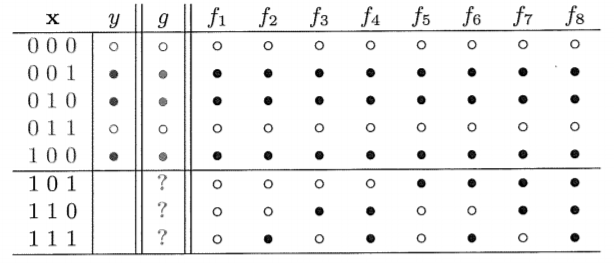
\includegraphics[width=0.75\textwidth]{FactorTable.PNG}
\caption{Table courtesy of the textbook \textit{Learning from Data}.}
\label{FactorTable}
\end{center}
\end{figure}

From the table in the book, we can see that there are 8 possible  f functions. Letting open circles equal 0 and shaded circles equal 1, we have the same table as the problem. We can now see that filling in any three values of g will always have 1 possible f function that matches completely, 3 that have 2 matches, 3 that only have 1 match, and 1 that has no match. So theoretically all possible g functions should have the same score \textbf{(E)}.

\section*{Problem 7}

\textbf{(B)} - The typical number of iterations based on my code was around 10, so 15 is the closest. It makes sense because there are only 10 points, so it shouldn't take too many iterations.

\section*{Problem 8}

\textbf{(C)} - The accuracy of the algorithm was around 90\%  with my code which makes sense because there are only 10 points, so it's easier to find a w that classifies everything in the data set correctly, but isn't the same as f.

\section*{Problem 9}

\textbf{(B)} - My code took around 90 iterations each time which makes sense because it should take more iterations than when you only have 10 data points.

\section*{Problem 10}

\textbf{(B)} - The accuracy of the algorithm this time was around 98.6\% which makes sense because with more points, in order for w to correctly classify the entire data set it must be closer to f.

\end{document}
	% line of code telling latex that your document is ending. If you leave this out, you'll get an error
